\documentclass[12pt,a4paper]{article}
\usepackage[utf8]{inputenc}
\usepackage[frenchb]{babel}
\usepackage[T1]{fontenc}
\usepackage{amsmath}
\usepackage{amsfonts}
\usepackage{amssymb}
\usepackage{graphicx}
\usepackage{subcaption}
\usepackage{lastPage}

\usepackage{fancyhdr}
\usepackage[left=2cm,right=2cm,top=2cm,bottom=2cm]{geometry}

\pagestyle{fancy}
\setlength{\unitlength}{1mm}
\addtolength{\headheight}{1.5\baselineskip}
\renewcommand{\headrulewidth}{0.6pt}
\renewcommand{\footrulewidth}{0.4pt}
\fancyfoot{}
\rhead{
\includegraphics[width=0.7cm]{ENS.png}}
\chead{\today}
\rfoot{\thepage\  / \pageref{LastPage}}
\lfoot{Adrien Vigné}
\cfoot{ Outils numériques - Mécanique générale}

\csname @addtoreset\endcsname{section}{part}

\begin{document}

\begin{titlepage}
\centering
{\scshape \LARGE École normale Supérieure de Rennes \par}
\vspace{1cm}
{\huge \LARGE  Outils numériques - Mécanique générales \par}
\vspace{1cm}
{\LARGE \itshape Adrien Vigné \par}
\vspace{1cm}
{\LARGE \itshape Étudiant 1\up{ère} année Département Mécatronique \par}
\vspace{1cm}
{\LARGE \today \par}
\vspace{5cm}

\includegraphics[scale=0.5]{ENS.png}

\end{titlepage}

\tableofcontents

\newpage

\part*{Introduction:} 
La mécanique est une partie important de l'étude de la mécatronique. L'objectif de cette outils numérique de mécanique générale est de prendre en main un environnement de modélisation multi-physiques \textsc{Matlab/Simulink}. Au travers de la bibliothèque \textsc{Simscape} qui permet la modélisation multi-physiques notamment la partie mécanique qui nous intéresse pour ce cours (module \textit{Multibody}). Dans un première temps on cherche à créer un système mécanique puis à modéliser deux systèmes mécaniques simples.Pour finir on modélise un robot SCARA.

\part{Construction d'un système mécanique} 
\paragraph*{Objectifs:}
Le but de cette première partie est de comprendre la réalisation d'une pièce et le rôle des blocs de base de la modélisation sous \textsc{Matlab/Simulink}.
\section{Création d'une pièce dans le monde de simulation}

Une fois l'environnement de modélisation ouvert ("smnew") on se retrouve avec des blocs fixant les conditions des résolution(figure \ref{solveur} / \ref{reférentiel} /\ref{param_mecanique}) et d'autres paramétrant les liens entre les solides (figure \ref{changement_base}) ainsi que les blocs représentants les solides eux-mêmes(figure \ref{solide}).

\begin{figure}[h!]
\centering
\begin{minipage}[c]{0.3\linewidth}
\centering
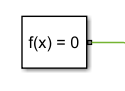
\includegraphics[scale=0.7]{solveur.png}
\caption{Paramètres du solveur}
\label{solveur}
\end{minipage} \hfill
\begin{minipage}[c]{0.3\linewidth}
\centering
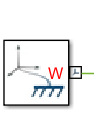
\includegraphics[scale=0.5]{repere.png}
\caption{Référentiel de la modélisation}
\label{reférentiel}
\end{minipage} \hfill
\begin{minipage}[c]{0.3\linewidth}
\centering
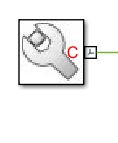
\includegraphics[scale=0.5]{param.png}
\caption{Paramètres mécanique}
\label{param_mecanique}
\end{minipage} 
\end{figure}

\begin{figure}[h!]
\centering
\begin{minipage}[c]{0.4\linewidth}
\centering
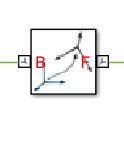
\includegraphics[scale=0.7]{changement.png}
\caption{Changement de base}
\label{changement_base}
\end{minipage} \hfill
\begin{minipage}[c]{0.4\linewidth}
\centering
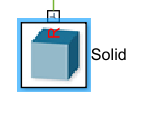
\includegraphics[scale=0.75]{solid.png}
\caption{Représentation des solides}
\label{solide}
\end{minipage} 
\end{figure}

On peut définir les paramètres des solides dans la boite à dialogue du bloc solid à l'aide de variables définie dans l'environnement \textsc{Matlab}(L,W,H,rho) (figure \ref{géométrie})

\begin{figure}[h!]
\centering
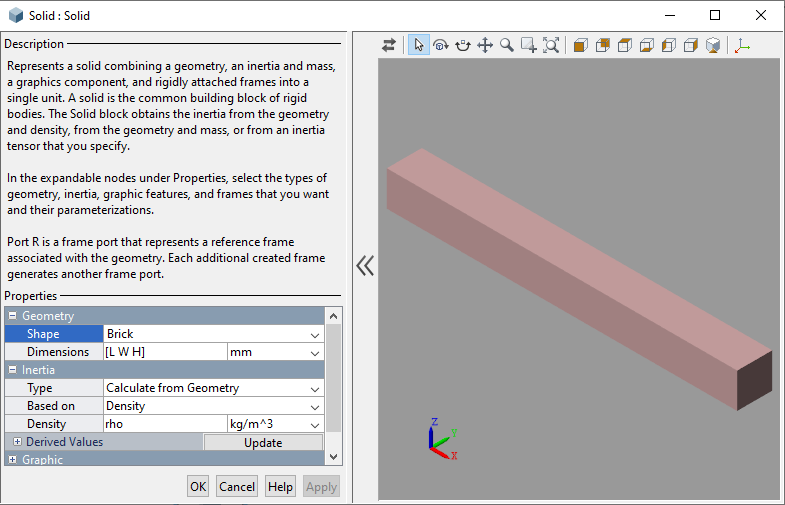
\includegraphics[width=0.8\linewidth]{geometrie.png}
\caption{Fenêtres de modification des solides}
\label{géométrie}
\end{figure}

\newpage

Dans cette partie on a donc créer un solide avec une géométrie simple et placer à l'aide de changement de base des repères d'un cote et de l'autre du solide. On peut maintenant utiliser cette ensemble comme une brique élémentaire pour le reste du TP en y appliquant un masque.



\section{Positionner une pièce par rapport à une autre}

En utilisant le bloc crée dans la partie précédente on cherche à former un parallélogramme. On place pour ceci des changement de base entre chaque pièce en définissant un angle nécessaire au parallélogramme dans chaque liaison(figure \ref{simulink_parallélograme}). On modifie 2 pièce sur 4 en changeant ces proportions et sa couleur afin de visualiser un parallélogramme (figure \ref{figure_parallélograme}).

\begin{figure}[h!]
\centering
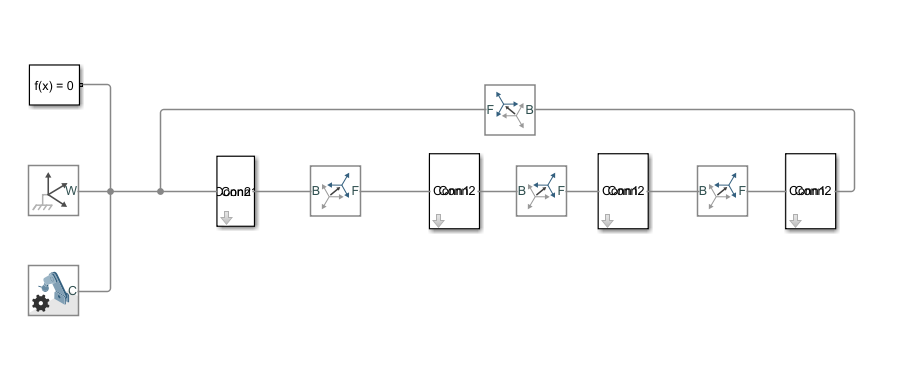
\includegraphics[scale=0.5]{parallelo.png}
\caption{Bloc élémentaire et changement de base sous simulilnk}
\label{simulink_parallélograme}
\end{figure}

\begin{figure}[h!]
\centering
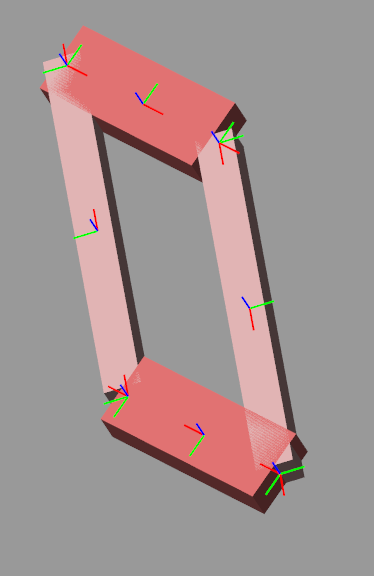
\includegraphics[scale=0.5]{figure_paralallelo.png}
\caption{Parallélogramme créer à partir des liaisons et blocs de la partie de la partie précédente}
\label{figure_parallélograme}
\end{figure}
 
Dans cette partie, on a former un assemblage de solide à l'aide des blocs que l'on a vu ou creer dans la première partie. L'assemblage de pièce étant maintenant fait on va chercher à actionner l'ensemble pour continuer dans l'optique de la découverte de la modélisation mécanique.

\section{Ajout d'un degré de liberté pouvant être actionné}
En mécanique on s'intéresse aussi au actionneur des ensembles de solides c'est que l'on va faire dans cette partie. pour cela on remplace les liaisons fixes par des liaisons actionnable définie dans la bibliothèque. On choisit des liaisons pivot et on définit la position initiale comme la position du parallélogramme précédente. On actionne une seul des liaisons avec un couple constant de $0.1  N.m$ 

\begin{figure}[h!]
\centering
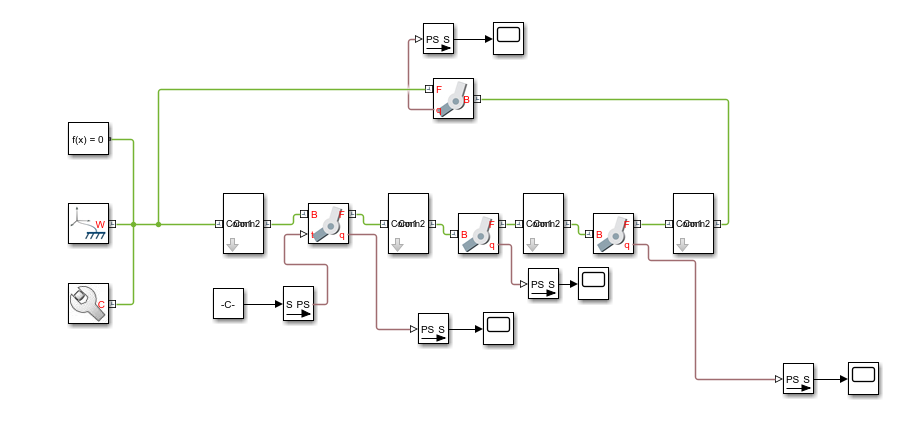
\includegraphics[scale=0.8]{motorise.png}
\caption{Parallélogramme motorisé}
\label{motorise_parallélograme}
\end{figure}
 
Dans les liaison pivot on peut récupérer les informations de posotion ,vitesse et accélération ainsi que le couple.On peut actionner cette liaison avec un couple ou par une commande de position, il est aussi possible de définir des frottements interne à la liaison.

Par construction les solides parallèles 2 à 2 le restent pendant tout le déplacement.

\section{Conclusion}
Cette activité a permis de découvrir la modélisation ainsi que la création d'un ensemble simple et de l'actionner à l'aide de liaison prédéfinie.On peut donc facilement créer un solide paramétrer par un programme \textsc{Matlab} et récupérer la position des éléments ou les efforts dans les liaisons pour un pré-dimensionnement simple par exemple.

\part{Modélisation de systèmes mécaniques simples}


\paragraph*{Objectifs :}
L'objectif ici est de modéliser des systèmes mécaniques simples après avoir étudier la création d'un modèle simple on rajouter des éléments supplémentaire comme des ressorts et des frottements. 
\section{Modélisation d'un système masse-ressort}
\paragraph*{Objectifs:}
L'objectif de cette partie est de modéliser un système masse-ressort amortisseur et de vérifier si la mise en équation correspond à la solution temporelle tracé avec le logiciel.


Pour un système masse-resoort la mise en équation donne :

\[ \ddot{x}+\dfrac{B}{m} \cdot \dot{x} + \dfrac{k}{m} \cdot x = \dfrac{k \cdot l_{0}}{m} \]
Dont la solution est : 
\[ x(t) = e^{-t/\tau} \cdot \left((x_{0}-l_{0}) \cdot \cos(\dfrac{\sqrt{\Delta}}{2}\cdot t)+ \dfrac{(x_{0}-l_{0}) B}{\sqrt{\Delta} m} \cdot \sin(\dfrac{\sqrt{\Delta}}{2}\cdot t) \right) + l_{0} \]

Avec \[\Delta = (\dfrac{B}{m})^2 - \dfrac{4 k}{m}\] et \[\tau = \dfrac{2 m }{B}\]
$x_0$ la longueur initiale, $l_0$ la longueur à vide du ressort 
\newline

On le modélise sous \textsc{simulink} l'ensemble masse-ressort a l'aide d'un bloc ressort et amortisseur en parallèle avec une liaison glissière puis d'un masse ponctuelle car ici la géométrie du solide n'intervient pas dans la modélisation mis en équation(figure \ref{masse}).

\begin{figure}[h!]
\centering
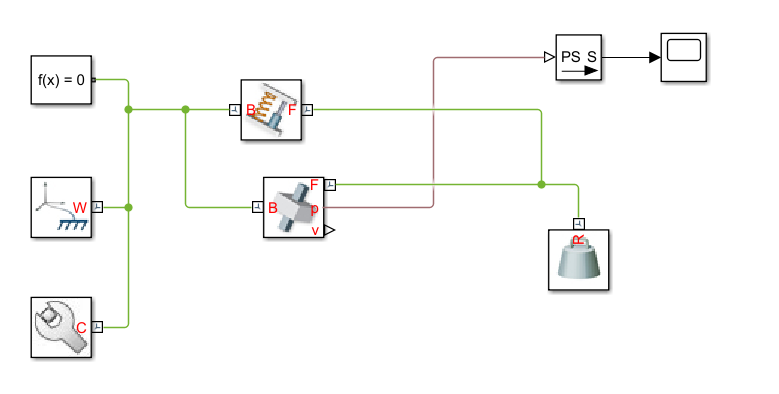
\includegraphics[scale=0.6]{masse.png}
\caption{Modèle du système masse-ressort amortisseur}
\label{masse}
\end{figure}
\newpage
On peut vérifier la solution de l'équation en regardant le tracé de la position en fonction du temps de la masse (figure \ref{masse_ressort}).

\begin{figure}[h!]
\centering
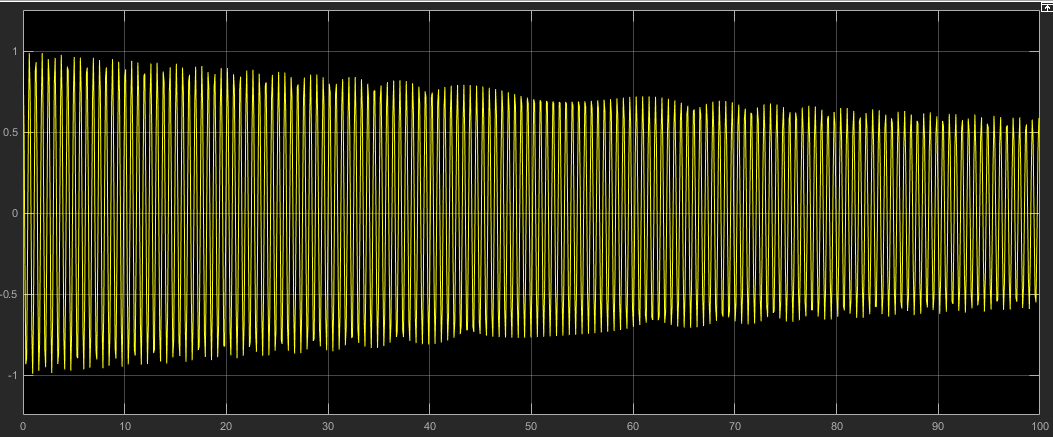
\includegraphics[scale=0.6]{masse_resort.png}
\caption{Position de la masse en fonction du temps }
\label{masse_ressort}
\end{figure}

On remarque bien l'atténuation des oscillations comme cela est décrit dans l'équation de la solution.
\newline
\paragraph*{Conclusion:}
On a donc bien décrit un système masse-ressort conforme à l'équation théorique sous l'environnement de modélisation \textsc{Simulink}

\section{Modélisation d'un pendule}
\paragraph*{Objectif:} Dans cette partie on veut modéliser un pendule dans lequel la corde est rigide. 

On trouve avec la mise en équation en considérant uniquement la gravité et la tension de la corde: 

\[ \ddot{\theta} + \dfrac{g}{l} \cdot \sin(\theta) = 0 \]

En faisant l'approximation des petits angles. On obtient l'équation :
\[ \ddot{\theta} + \dfrac{g}{l} \cdot \theta = 0 \]

Avec l la longueur de la corde.

On peut modéliser ceci sous \textsc{Simulink} en utilisant un changement de base pour positionner le pendule,une liaison pour le degré de liberté du système et une masse ponctuelle car on ne tient pas compte des frottements(figure \ref{pendule}).

\begin{figure}[h!]
\centering
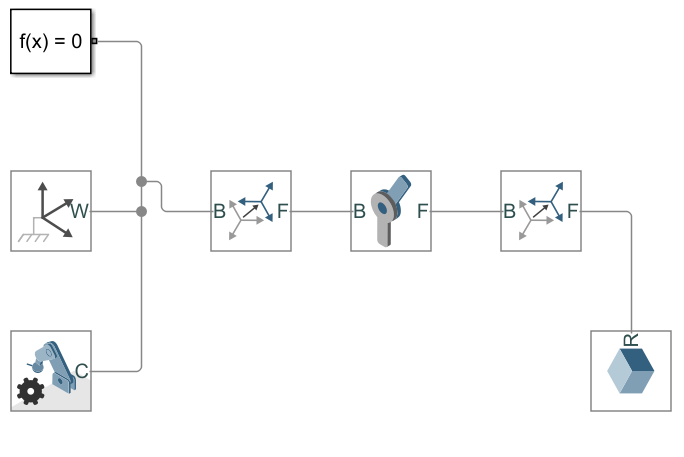
\includegraphics[scale=0.6]{pendule.png}
\caption{Modèle du pendule}
\label{pendule}
\end{figure}

On peut observer si l'hypothèse des petits angles utilisée dans la mise en équation est valable en traçant la position du pendule en fonction du temps (figure \ref{trace_pendule}) avec pour conditions initiales un angle de 10\degres.

\begin{figure}[h!]
\centering
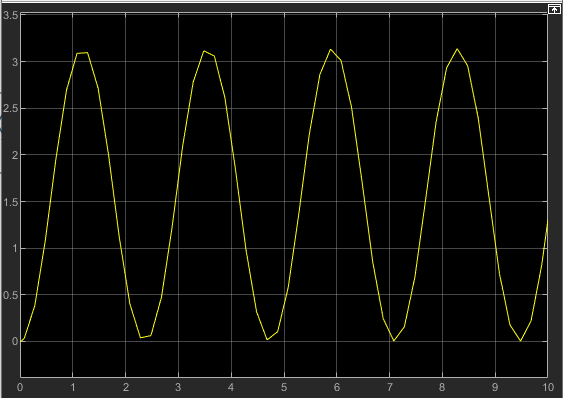
\includegraphics[scale=0.6]{trace_pendule.png}
\caption{Position du pendule en fonction du temps}
\label{trace_pendule}
\end{figure}

On peut donc voir ici que l'hypothèse des petits angle est valable pour cette modélisation dans ces conditions car la tracé correspond bien à la solution dans cette approximation.

\paragraph*{Conclusion :}
Dans cette partie on a pu modéliser un système pendule et vérifier si l'approximation faite dans la mise en équation était valable. 

\section{Conclusion:} 
On a pu modéliser des systèmes mécaniques plus complexe que dans la partie précédente en utilisant les modules disponibles dans la librairie et ceci à permit de vérifier la mise en équation et les hypothèses posés.

\part{Modélisation du robot SCARA}
\section{Choix de modélisation et hypothèses}
\subsection{Modélisation simplifier}
\subsection{Hypothèses}
\section{Modèle \textsc{Simulink}}
\subsection{Commande en trapèze de vitesse}
\subsection{Choix des moteurs}
\section{Evolution du système}
\subsection{Optimiation de l'inertie}
\subsection{Monteur CC et aservissement}




 
\end{document} 
